\documentclass{article}

\usepackage{amsmath, amsthm, amssymb, amsfonts}
\usepackage{physics}
\usepackage{thmtools}
\usepackage{graphicx}
\usepackage{setspace}
\usepackage{geometry}
\usepackage{float}
\usepackage{hyperref}
\usepackage[utf8]{inputenc}
\usepackage[english]{babel}
\usepackage{framed}
\usepackage[dvipsnames]{xcolor}
\usepackage{tcolorbox}
\usepackage{tikz-cd}

\colorlet{LightGray}{White!90!Periwinkle}
\colorlet{LightOrange}{Orange!15}
\colorlet{LightGreen}{Green!15}
\colorlet{LightBlue}{Blue!10}

\newcommand{\HRule}[1]{\rule{\linewidth}{#1}}

\declaretheoremstyle[name=Theorem,]{thmsty}
\declaretheorem[style=thmsty,numberwithin=section]{theorem}
\tcolorboxenvironment{theorem}{colback=LightGray}

\declaretheoremstyle[name=Proposition,]{prosty}
\declaretheorem[style=prosty,numberlike=theorem]{proposition}
\tcolorboxenvironment{proposition}{colback=LightOrange}

\declaretheoremstyle[name=Definition,]{defsty}
\declaretheorem[style=defsty,numberlike=theorem]{definition}
\tcolorboxenvironment{definition}{colback=LightGreen}

\declaretheoremstyle[name=Corollary,]{corsty}
\declaretheorem[style=corsty,numberlike=theorem]{corollary}
\tcolorboxenvironment{corollary}{colback=LightBlue}

\setstretch{1.2}
\geometry{
    textheight=9in,
    textwidth=5.5in,
    top=1in,
    headheight=12pt,
    headsep=25pt,
    footskip=30pt
}
%-------------------------------------------------------------------------------
% Some useful macros and defs
%-------------------------------------------------------------------------------

\def\nn{\nonumber} 
\def\pa{{\partial}}
\def\f{\frac}
\def\l{\left}
\def\r{\right}
\def\es{\emptyset}
\def\R{\mathbb{R}}
\def\C{\mathbb{C}}
\def\N{\mathbb{N}}
\def\Z{\mathbb{Z}}
\def\Q{\mathbb{Q}}
\def\H{\mathbb{H}}
\def\e{\epsilon}
\def\a{\alpha}
\def\b{\beta}
\def\g{\gamma}
\def\p{\phi}
\def\d{\delta}
\def\Ker{\text{Ker}}
\def\aut{\text{Aut}}
\def\mod{\text{Mod}}
\def\diff{\text{Diff}}
% ------------------------------------------------------------------------------

\begin{document}

% ------------------------------------------------------------------------------
% Cover Page and ToC
% ------------------------------------------------------------------------------

\title{ \normalsize \textsc{}
		\\ [2.0cm]
		\HRule{1.5pt} \\
		\LARGE \textbf{\uppercase{Automorphisms of Hyperbolic Surfaces}
		\HRule{2.0pt} \\ [0.6cm] \LARGE{Notes made for thesis project} \vspace*{10\baselineskip}}
		}
\date{Updated on: \today}
\author{\textbf{Manvendra Somvanshi}}

\maketitle
\newpage

\tableofcontents
\newpage

% ------------------------------------------------------------------------------
\section{Torus and it's Automorphisms}
\begin{definition}
Define the torus, $T^2$ as the quotient space $\R^2/\Z^2$ where two points are equivalent if their difference is in $\Z^2$.
\end{definition}
Note that this is homeomorphic to the usual definition $S^1 \times S^1$. The universal covering space of $T^2$ is $\R^2$ and it's fundamental group is $\Z^2$. We identify the equivalance class of the closed curve $\gamma(t)$ based at $[(0,0)]$ with $\tilde{\g}(1)\in \Z^2$, where $\tilde{\g}$ is the lift of $\g$ based at $(0,0)$ in $\R^2$. This map, from $\pi_1(T^2) \to \Z^2$ is a bijection since $\R^2$ is simply connected (see theorem 54.4 on pg 345 in \cite{munkres}).\\

  Automorphisms on the torus correspond to elements in $GL_2(\Z)$. Suppose that $\p:T^2 \to T^2$ is an automorphism then it induces a map $\p_* :\pi_1(T^2) \to \pi_1(T^2)$ which is an isomorphism. Since isomorphisms of $\Z^2$ are just invertible integer matrices. These are just $GL_2(\Z)$ which is the same as matrices with determinant $\pm 1$. On the other hand any $A\in GL_2(\Z)$ will induce an automorphism $\p_A$ on $T^2$ where the mapping is just $[(x,y)] \mapsto [(x,y)A^t]$. The automorphism is orientation preserving if and only if the corresponding matrix $A$ has positive determinant, i.e. $1$.
\begin{proposition}
  The correspondence $\aut(T^2) \to GL_2(\Z)$ is a homomorphism. Moreover if $A$ is in $GL_2(\Z)$ then $(\p_A)_* = A$; i.e. the correspondence is surjective.
\end{proposition}
\begin{proof}
  Since $\l(\phi\circ \psi\r)_*[\g] = [\p\circ\psi \circ \g] = \p_*\circ \psi_*([\g])$ it follows that the map $\p \mapsto \p_*$ is a homomorphism. Let $A$ be $GL_2(\Z)$, then $\p_A$ is well defined automorphism of the torus. Now $\p_{A*}$ acts on $(m,n)\in \Z^2$ in the following way: $(m,n)$ corresponds to the unique class $[\g]$ where $\tilde{\g}(1) = (m,n)$, so the action is given by $\p_{A*}(m,n) = \widetilde{\p_A\circ\gamma}(1)$. Since $\p_A \circ \gamma(t) = \g(t)A^t$, the lifting of this at $(0,0)$ will be just $\tilde{\g}(t) A^t$ (since liftings are unique and this is a lift). Thus $\p_{A*}(m,n) = (m,n)A^t$. Thus $\p_{A*}$ just corresponds to the matrix $A$ in $GL_2(\Z)$.
\end{proof}
Let $A$ be a matrix in $SL_2(\Z)$ and $\p_A$ be the corresponding orientation preserving automorphism, then we can classify $\p_A$ by looking at the properties of the matrix $A$. The characteristic equation of such a matrix is given by $x^2 - \tau x + 1$, where $\tau$ is the trace. We break this into three possibilities:
\begin{enumerate}
  \item $\tau = 0, \pm 1$. In this case the characteristic equation is $x^2 +1$, $x^2-x+1$, or $x^2 + x+ 1$. Thus the eigenvalue are complex in this case. Using Cayley-Hamilton theorem $A$ solves its characteristic equation. In each case we have $A^4 = I$, $A^6=I$, or $A^3=I$ resp.; hence $A^{12} = I$ in each case. Thus the map $\p_A$ is also a finite order map. In this case $\p_A$ is said to be periodic.
  \item $\tau = \pm 2$. In this case the characteristic is $(x\pm 1)^2$. Both eigenvalues are either $1$ or both are $-1$ respectively. Eigenvector of $A$ is integeral and thus correspond to (class of) closed curves on $T^2$. The map preserves the (equivalance class of the) curve (reverses the direction when $\tau = -2$) represented by the eigenvector. No other curve is preserved under the map. These are powers of the Dehn Twists in $C$. 
    \begin{definition}
      A Dehn Twist along a curve $\g$ is defined in the following way: Let $A$ be a regular neighborhood containing $C$ such that $A$ is homeomorphic to an annulus parametrized as $(r,\theta)$. The the extension of the homeomorphism $\p(r,\theta) = (r,\theta + 2\pi r)$ to the whole of the torus (via characteristic function on $A$), is called the Dehn twist.
    \end{definition}
    Matrices corresponding to Dehn twists which preserve the curves corresponding to $(1,0)$ and $(0,1)$ are
    \begin{align*}
      T = \begin{pmatrix}
        1 & 0\\ 1 & 1
      \end{pmatrix}
      \And
      S = \begin{pmatrix}
        1 & -1\\ 0 & 1
      \end{pmatrix}
    \end{align*}
    respectively. \textit{These matrices generate $SL_2(\Z)$ as a group}.
    \begin{figure}
      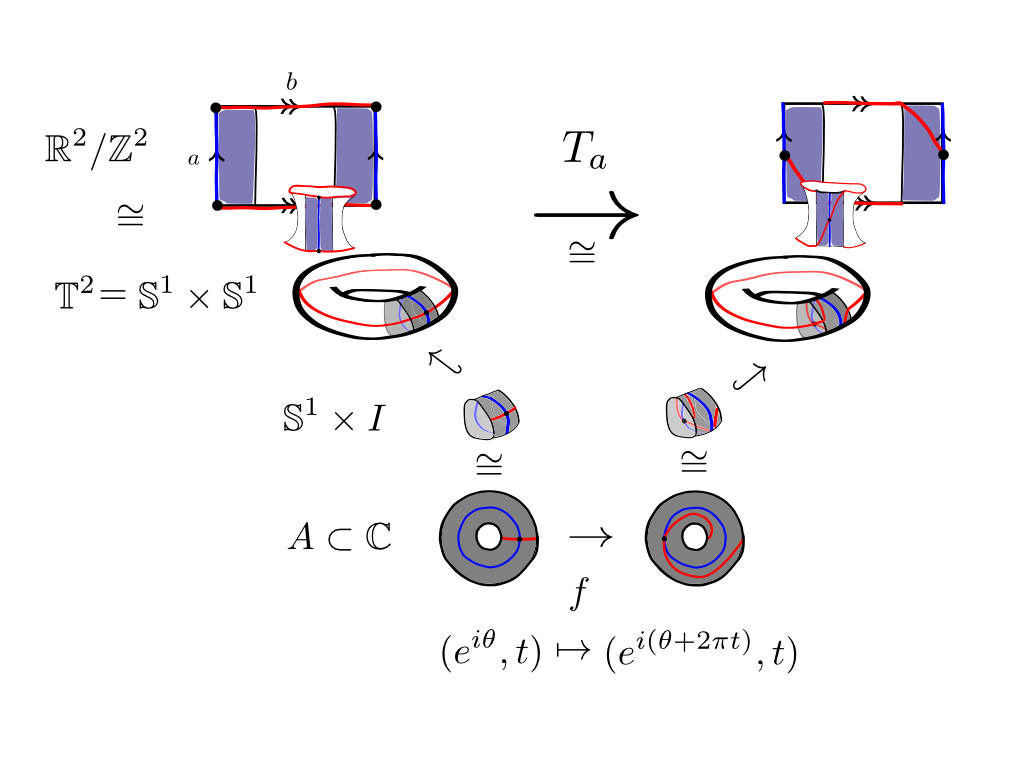
\includegraphics[scale=0.5]{figures/Dehn_twist_for_the_torus.png}
      \caption{Dehn twist along the class of curves represented by $(1,0)$ (blue). The red curve is in the class represented by $(0,1)$. Source of image is wikipedia.}
    \end{figure}
  \item $|\tau| > 2 $. In this case the eigenvalues are distinct reals. The eigenvalues satisfy the relation $\lambda_1\lambda_2 = 1$. Let $|\lambda_1|> 1$. Thus the eigenvalues are of the form $\lambda, 1/\lambda$. Let $v_1,v_2$ be the corresponding eigenvectors. Think of these as elements of $T_{p}(\R^2/\Z^2)$ (tangent space). Consider the curves $\g_i = v_i t $. The action of the map $\p_A$ on $\g_1$ expands it by a factor of $\lambda$ and on $\g_2$ it contracts it by $\lambda^{-1}$. Such maps are called \textit{Anosov Maps}.
\end{enumerate}

\section{Hyperbolic Plane}
\begin{definition}
  The upper half plane model of the hyperbolic plane is the set of all points in $\C$ with positive imaginary part, $\Im(z)> 0$ with the metric given by
  \begin{align*}
    \dd s^2 = \frac{(\dd x^2 + \dd y^2)}{y^2}
  \end{align*}
  We denote this by $ \mathbb{H}$. 
\end{definition}

\begin{definition}
  The hyperbolic length of a piecewise differentiable curve $\g:[0,1]\to \mathbb{H}$ is given by
  \begin{align*}
    h(\g) = \int_0^1 \frac{|\dot{\g}(t)|}{\Im(\g(t))} \dd t
  \end{align*}
  The distance between two points $z_1, z_2$ is given by,
  \begin{align*}
    \rho(z_1,z_2) = \inf_{\g} h(\gamma),\ \g(0) =z_1 \qq{and} \g(1) = z_2
  \end{align*}
  this is well defined since $\C$ is path connected.
\end{definition}
\begin{proposition}
  $\rho$ is a metric.
\end{proposition}
\begin{proof}
  Suppose that $\rho(z_1,z_2) = \ell_1$ and $\rho(z_2,z_1) = \ell_2$. Now let $\gamma$ be any curve from $z_2$ to $z_1$. Then $\g(1-t)$ is a curve from $z_1$ to $z_2$ and since $h(\g) = h(\g(1-t))\geq \ell_1$ it follows that $\ell_1$ is also a lower bound and we must have $\ell_1 \leq \ell_2$. Repeating the same in the opposite direction we have $\ell_2\leq \ell_1$. Hence $\rho$ is symmetric.\\

  Let $z_1,z_2, z_3$ be three points. Represent curves from $z_1 \to z_2$ by $\g$, $z_2\to z_3$ by $\sigma$ and $z_1\to z_3 by \tau$. Given any $\g$ and $\sigma$ we can construct a curve from $z_1$ to $z_3$ in following way
  \begin{align*}
    \tau(t) = \g * \sigma(t) = \begin{cases}
      \g(2t),\ 0\leq t\leq 1/2\\
      \sigma(2t-1),\ 1/2 \leq t\leq 1.
    \end{cases}
  \end{align*}
  The length $h(\g*\sigma) = h(\g) + h(\sigma)$ (linearity and change of variables). It follows
  \begin{align*}
    \inf_\tau h(\tau) &\leq \inf_{\g, \sigma} h(\g*\sigma) = \inf_\g h(\g) + \inf_\sigma h(\sigma)\\
    \implies \rho(z_1,z_3) &\leq \rho(z_1,z_2) + \rho(z_2,z_3).
  \end{align*}
  Hence $\rho$ satisfies triangle inequality.\\

  Clearly $\rho(z,z) = 0$. Let $z_1, z_2$ be two points and $\g$ be a curve between them. Then
  \begin{align}
    h(\g) &= \int_0^1 \f{|\dot{\g}|}{\Im(\g)} \dd t \geq \abs{\int^1_0 \f{\dot{\g}}{\Im(\g)} \dd t} \nonumber\\
          &> \f{1}{M}\abs{\int^1_0 \dot{\g}\dd t} = \f{1}{M} |z_2-z_1|
  \end{align}
  Where $M = \sup_{t\in [0,1]}(Im(\g(t)))$ (this is well defined since its a continuous function on a compact interval). This completes the proof.
  Suppose $\rho(z_1,z_2) = 0$ then $h(\g)< 0$ and hence $|z_1 - z_2| < 0$. Hence $z_1 = z_2$.
\end{proof}
\begin{proposition}
  The set of all Mobius transforms from $\C\to \C$ of the form
  \begin{align*}
    z \mapsto \f{az+b}{cz+d},\ a,b,c,d\in \R\ ad-bc =1
  \end{align*}
  form a group, under composition. This group is isomorphic to $PSL_2(\R) = SL_2(\R)/\{\pm I\}$.
\end{proposition}
\begin{proof}
  The first part is trivial. For the second consider the map from $SL_2(\R)$
  \begin{align*}
    \begin{pmatrix}
      a&b\\c&d
    \end{pmatrix} \mapsto \l(z\mapsto \f{az+b}{cz+d}\r)
  \end{align*}
  This is clearly surjective. Suppose that
  \begin{align*}
    \f{az+b}{cz+d} = z \implies -cz^2 + (a-d)z + b = 0 \implies c = 0,\ a=d,\ b=0.
  \end{align*}
  Since $ad-bc=1$ it follows that $a = \pm 1$. Hence $\ker$ of the map is just $\pm I$.
\end{proof}
Note that any Mobius transformation in $PSL_2(\R)$ can be written by composing the functions $z\mapsto az$, $z\mapsto z+b$, $z\mapsto -1/z$.
\begin{proposition}
  The metric topology of $\H$ is equivalent to the subspace topology induced from $\C^2$.
\end{proposition}
\begin{proof}
  Consider the two points $z,w\in\H$. Consider the curve $\g(t) = (z-w)t + w$. By definition
  \begin{align*}
    \rho(z,w) \leq \int^1_0 \f{|\dot{\g}|}{\Im(\g)} \dd t = |z-w| \int^1_0 \f{\dd t}{(y-v)t+v} \leq |z-w| \int^1_0 \f{\dd t}{\min\{y,v\}} = \f{|z-w|}{\min\{y,v\}}  
  \end{align*}
  Where $\Im(z) = y$ and $\Im(w) = v$. Hence $\rho(z,w) \leq K_w |z-w|$ for some $K_w>0$. From (1) we already know that
  \begin{align*}
    |z-w| \leq M \rho(z,w) 
  \end{align*}
  Hence the metrics are equivalent. 
\end{proof}
This is an important result since we can just check the continuity of functions under the regular metric. This helps reduce calculations.
\begin{theorem}
  $PSL_2(\R)$ acts on $ \mathbb{H}$ by homeomorphisms.
\end{theorem}
\begin{proof}
  Suppose $z\in\H$ and
  \begin{align*}
    w = \f{az+b}{cz+d}
  \end{align*}
  then
  \begin{align*}
    w-\bar{w} &= \f{az+b}{cz+d} - \f{a\bar{z}+b}{c\bar{z}+d}\\
              &= \f{z-\bar{z}}{|cz+d|^2} > 0
  \end{align*}
  Thus points on $\H$ are mapped to $\H$ itself. Since mobius transformations are bijective, continuous, and the inverse again is a mobius transformation it follows that it is a homeomorphism on $\H$. 
\end{proof}
\begin{theorem}
  $PSL_2(\R)$ is isomorphic to a subgroup of the isometry group of $\H$.
\end{theorem}
\begin{proof}
  Let $z,w\in \H$ and $T\in PSL_2(\R)$ be a mobius transformation $(a,b,c,d)$. Let $\g$ be a curve from $z$ to $w$ then $\sigma(t) = T(\g(t))$ is a curve from $Tz$ to $Tw$. Since
  \begin{align*}
    \dot{\sigma}(t) = \f{\dot{\g}}{(c\g + d)^2},
  \end{align*}
  and
  \begin{align*}
    \Im{\sigma(t)} = \f{\Im{\g}}{|c\g(t)+d|^2}
  \end{align*}
  it follows that
  \begin{align*}
    h(\sigma) = h(\g).
  \end{align*}
  Since $T$ is bijective there is a bijective correspondence between curves from $z$ to $w$ and curves from $Tz$ to $Tw$. Thus they have the same infimum, meaning that $\rho(w,z) = \rho(Tw,T,z)$. 
\end{proof}
\begin{definition}
  Geodesics are curves with the shortest length between any two points in a metric space.
\end{definition}
\begin{theorem}
  The geodesics in $\H$ are straight lines and semi circles perpendicular to the real axis. Moreover, between any two points in $\H$ there exists a unique geodesic.
\end{theorem}
\begin{proof}
  Consider the two points $z = a_0 + ia$ and $w = a_0 + ib$ in $\H$. For any curve $\g(t) = x(t) + iy(t)$ between these points,
  \begin{align}
    h(\g) &= \int^1_0 \f{\sqrt{\dot{x}^2 + \dot{y}^2}}{y(t)} \dd t \nn\\
          &\geq \int^1_0 \f{|\dot{y}|}{y(t)}\dd t \nn\\
          &\geq \abs{\int^1_0 \f{\dot{y}}{y} \dd t} \nn \\
          &= \abs{\log(\f{b}{a})}
  \end{align}
  But since the curve $\g_0(t) = i(b-a)t + ia + a_0$ also has the length $|\log(b/a)|$ it follows that $\rho(z,w) = |\log(b/a)|$. The geodesic, $\g_0$, in this case is a straight line perpendicular to $\R$.\\

  Now consider any two points $z_1,z_2\in \H$. Then there is a unique circle which passes through $z_1,z_2$ and is perpendicular to the real line: $|z-a| = r$ where
  \begin{align*}
    a = \f{|z_1|^2 - |z_2|^2}{2(\Re(z_1-z_2))} \And r = |z_1 - a|. 
  \end{align*}
  There also exists a $T\in PSL_2(\R)$ which maps the above semi-circle in $\H$ to the positive imaginary line. Explicitly this is:
  \begin{align*}
    T = \f{1}{\sqrt{2r}}\begin{pmatrix}
      1 & -a-r \\ 1 & -a +r 
    \end{pmatrix}
  \end{align*}
  Suppose that $z$ lies on the semi-circle, then $z-a = re^{i\theta}$. Thus under the transformation
  \begin{align*}
    T(z) = \f{e^{i\theta}-1}{e^{i\theta}+1} \in i\R^+
  \end{align*}
  Hence the semi circle gets mapped to the imaginary axis, which is a geodesic. Since $T$ is an isometry it follows that the semicircle is also a geodesic. The uniqueness follows from the fact that for any curve other than the straight line the inequality in $2$ is strict, and hence only the straight line achives the minimum length. By isometry argument it generalizes to the aribtrary case.
\end{proof}
\begin{definition}
  The set of points on the unique geodesic connecting $w$ and $z$ is represented by $[w,z]$.
\end{definition}
\begin{corollary}
  Let $z,w,\xi\in \H$ then,
  \begin{align*}
    \rho(z,w) = \rho(z,\xi) + \rho(\xi,w)
  \end{align*}
  if and only if $\xi\in [z,w]$.
\end{corollary}
\begin{proof}
  Suppose that $\xi\in [z,w]$. Then the geodesic $\g$ from $z$ to $w$ on restriction gives a geodesic between $z$ and $\xi$, because if not then there is some other $\sigma$ between $z,\xi$ such that $h(\sigma) < h(\g|_{[z,\xi]})$, and then the curve
  \begin{align*}
    \tilde{\g}(t) = \begin{cases}
      \sigma(2t),\ 0\leq t\leq 1/2\\
      \gamma\big|_{[\xi,w]} (2t-1),\ 1/2\leq t\leq 1  
    \end{cases}
  \end{align*}
  has smaller length, in contradiction to the fact that $\g$ is the geodesic. Hence
  \begin{align*}
    \rho(z,w) = h(\g) = h(\g\big|_{[z,\xi]}) + h(\g\big|_{[\xi,w]}) = \rho(z,\xi) + \rho(\xi,w).
  \end{align*}
  Conversly, suppose that the equality holds. Let $\g_1,\g_2$ be the geodesics between $z,\xi$ and $\xi,w$ respectively. The concatenation as above defines a curve between $z$ and $w$, and
  \begin{align*}
    \rho(z,w) = \rho(z,\xi) + \rho(\xi,w) = h(\g_1) + h(\g_2) = h(\g_1*\g_2)
  \end{align*}
  Hence the concatenation is a geodesic. Thus $\xi\in [z,w]$.
\end{proof}
\begin{theorem}
  $PSL_2(\R)$ maps geodesics to geodesics.
\end{theorem}
\begin{proof}
  Since, as seen already in theorem 2.7, $h(T\g) = h(\g)$ for all $T\in PSL_2(\R)$ and curves $\g$ between $z,w$. Thus it follows trivially that if $\g$ is a geodesic then so is $T\g$ 
\end{proof}
\begin{definition}
  A cross ratio, denoted $(z_1,z_2;,z_3,z_4)$ is defined as
  \begin{align*}
    (z_1,z_2;z_3,z_4) = \f{(z_1 - z_2)(z_3-z_4)}{(z_1-z_4)(z_3-z_2)}
  \end{align*}
\end{definition}
\begin{proposition}
  Cross ratios are preserved under Mobius transformations.
\end{proposition}
\begin{proof}
  The transformation $T$, given by
  \begin{align*}
    T(z) = \f{z-z_2}{z-z_4} \f{z_3-z_4}{z_3 -z_2},
  \end{align*}
  maps $z_2\mapsto 0$, $z_4\mapsto \infty$, $z_3\mapsto 1$. $T(z_1)$ is exactly the cross ratio. Let $S$ be any mobius transformation then $TS^{-1}$ is the transformation which maps $Sz_2 \mapsto 0$, $Sz_4\mapsto \infty$, and $Sz_3\mapsto 1$. Hence $TS^{-1}(z) = (z,Sz_2; Sz_3, Sz_4)$. Hence $(Sz_1,Sz_2;Sz_3,Sz_4) = TS^{-1}(Sz) = T(z) = (z_1,z_2;z_3,z_4)$.
\end{proof}
\begin{theorem}
  Let $w,z\in \H$ and $\g$ be the geodesic between them. Extend $\g$ in both directions and let $w^*, z^*\in \R\cup \{\infty\}$ be the end points of the extended curve (semi-circle or straight line perpendicular to real axis) such that $z\in [z^*,w]$. Then
  \begin{align*}
    \rho(w,z) = \log(w,z^*; z,w^*)
  \end{align*}
\end{theorem}
\begin{proof}
  As seen before there exists a $T\in PSL_2(\R)$ such that $T$ maps the extended $\g$ to the imaginary axis. Explicitly such a $T$ is
  \begin{align*}
    T(\xi) = i\f{\xi-z^*}{\xi-w^*}\cdot \f{z-w^*}{z-z^*} 
  \end{align*}
  this maps $z^*$ to $0$, $w^*$ to $\infty$, and $z$ to $i$. Note that the coefficient of $T$ are indeed all real, and it can be made determinant $1$ by multiplying and dividing by a real constant. And moreover,
  \begin{align*}
    T(w) = i\underbrace{\f{w-z^*}{w-w^*}\cdot \f{z-w^*}{z-z^*}}_{r}.
  \end{align*}
  $r$ must be greater than $1$ since $|z-w^*|>|w-w^*|$ and $|w-z^*|>|z-z^*|$ (since we choose $w$ to be closer to $w^*$ and $z^*$ is closer to $z$). The hyperbolic distance between $T(z)$ and $T(w)$ is $\log(r)$. Since $r = (ir,0;i,\infty) = (T(w), T(z^*); T(z), T(w^*)) = (w,z^*;z,w^*)$. Hence the statement of the theorem follows. 
\end{proof}

Now we describe the Poincare Disk model of the Hyperbolic plane. Consider the unit disk $\mathbb{D}$, and the map $\p:\H\to \mathbb{D}$
\begin{align*}
  \phi(z) = \f{iz+1}{z+i}
\end{align*}
Clearly $|\p(z)| = |z-i|/|z+i| < 1$ if and only if $z\in \H$. Also $\p$ maps the real line to the boundary of $ \mathbb{D}$. This map induces a distance $\rho^*$ on $ \mathbb{D}$ given by
\begin{align*}
  \rho^*(w,z) = \rho(\p^{-1}(w), \p^{-1}(z))
\end{align*}
It follows that,
\begin{align*}
  \rho^*(w,z) &= \inf_{\g} \int^1_0 \f{|\dv{\p^{-1}\circ \g}{t}|}{\Im(\p^{-1}\circ \g)} \dd t\\
          &= \inf_{\g} \int^1_0 \f{|\dv{\p^{-1}}{z}\big|_\g \dot{\g}|}{\Im(\p^{-1}\circ \g)} \dd t\\
          &= \inf_\g \int^1_0 \f{2|\dot{\g}(t)|}{1- |\g(t)|^2} \dd t
\end{align*}
This gives the metric on $ \mathbb{D}$ to be
\begin{align*}
  \dd s = \f{2|\dd z|}{1-|z|^2}.
\end{align*}
This model of the hyperbolic plane is called the Poincare Disk. The geodesics here are circles perpendicular to $ \mathbb{D}$ and diametric lines in $ \mathbb{D}$.
\begin{definition}
  Let the group of all $2\times 2$ matrices in $\R$ with determinant $\pm 1$ be denoted $S^*L_2(\R)$. Let $PS^*L_2(\R)$ be the group $S^*L_2(\R)/\{\pm I\}$.
\end{definition}
\begin{proposition}
  Let $z,w\in \H$. Then
  \begin{align*}
    \sinh(\f{1}{2} \rho(z,w)) = \f{|z-w|}{2\sqrt{\Im(z)\Im(w)}}
  \end{align*}
\end{proposition}
\begin{proof}
  Let $T$ be in $PSL_2(\R)$ then $T$ leaves the LHS invariant. It is straight forward to check that the RHS is also invariant. Suppose $z = ia$ and $w = ib$ ($b>a$) then we know that $\rho(ia,ib) = \log(b/a)$ and thus
  \begin{align*}
    \sinh(\f{1}{2}\rho(ia,ib)) = \f{b-a}{2\sqrt{ab}} = \f{|ib| - |ia|}{2\sqrt{\Im(ia)\Im(ib)}}
  \end{align*}
  Using the fact that there exists a $T$ which maps the geodesic between arbitrary $z,w$ to a geodesic between $ia,ib$; the result follows.
\end{proof}
\begin{theorem}
  The isometry group of $\H$ is isomorphic to $PS^*L_2(\R)$.
\end{theorem}
\begin{proof}
  Let $\p$ be any isometry. If $\xi\in [z,w]$ then
  \begin{align*}
    \rho(\p(z), \p(z)) = \rho(z, w) = \rho(z,\xi) + \rho(\xi,w) = \rho(\p(z), \p(\xi)) + \rho(\p(\xi), \p(w))
  \end{align*}
  Thus $\p(\xi) \in [\p(z), \p(w)]$. This means that isometries map geodesics to geodesics. Consider the positive imaginary line $I$ which is a geodesic. Then $\p(I)$ is also some geodesic. There exists a $g\in PSL_2(\R)$ such that $g$ maps $\p(I)$ to $I$. Without loss of generality we can assume $g(\p(i)) = i$ (since $g(\p(i)) = ai$, and dividing by $a$ we get another element of $PSL_2(\R)$) and that it maps $(0,i)$ and $(i,\infty)$ onto themselves (like in the previous theorem). Suppose that $g\circ\p(yi) = vi$ then
  \begin{align*}
    |\log(y)| = \rho(yi, i) = \rho(g\circ\p(yi), i) = |\log(v)|
  \end{align*}
  Either $v = y$ or $v = 1/y$, but since the intervals $(0,i)$ and $(i,\infty)$ are fixed it follows that $v = y$. Hence $g\circ\p$ fixes $I$. Let $\g\circ\p(x+iy) = u+iv$ then using the previous proposition on the points $x+iy$ and $it$ we get
  \begin{align*}
    \f{x^2 + (y-t)^2}{2y} = \f{u^2 + (v-t)^2}{2v} 
  \end{align*}
  dividing by $t^2$ and taking $t\to \infty$ we get $v = y$ and $x^2 = u^2$. Thus
  \begin{align*}
    g\circ\p(z) = z \qq{or,} -\bar{z}
  \end{align*}
  In the first case $\p$ is in $PSL_2(\R)$ and in the second case it is of the form
  \begin{align*}
    \p(z) = g^{-1}(-\bar{z}) = \f{a\bar{z} + b}{c\bar{z} + d},\ ad-bc = -1
  \end{align*}
  Thus $\p$ can be naturally mapped to an element of $S^*L_2(\R)$. The homomorphism part of the mapping follows easily, and the kernel of the map is $\{\pm I\}$. Thus the isometry group is isomorphic to $PS^*L_2(\R)$.
\end{proof}
Note that $PSL_2(\R)$ along with the map $h:z\mapsto -\bar{z}$ generates the isomoetry group. This means that the quotient space $PS^*L_2(\R)/PSL_2(\R)$ is just $\{PSL_2(\R), h\cdot PSL_2(\R)\}$ and thus has index $2$. This means that $PSL_2(\R)$ is normal in the isometry group.\\

The Riemannian metric of the Hyperbolic plane is induced by the inner product $\langle \cdot, \cdot \rangle: T_z\H \times T_z\H \to \R$ given by
\begin{align*}
  \langle \zeta_1, \zeta_2 \rangle = \f{1}{\Im(z)^2} \Re(\zeta_1 \bar{\zeta}_2)
\end{align*}
This is an inner product on $T_z\H$ over $\R$. This induces a norm $\|\cdot\|$ on $T_z\H$ defined as
\begin{align*}
  \|\zeta\| = \sqrt{\langle \zeta, \zeta \rangle} = \f{|\zeta|}{\Im(z)}
\end{align*}
Since all isometries of $\H$ are (real) differentiable, their pushforward gives a the map $\dd \p_z : T_z\H \to T_{\p(z)}\H$ 
\begin{align*}
  \dd\p_z(\zeta) = \f{\pm \zeta}{(cz+d)^2},\ \text{where},\ \p(z) = \f{az+b}{cz+d}, \And ad-bc = \pm 1. 
\end{align*}
The pushforward is norm preserving since
\begin{align*}
  \|\dd \p_z(\zeta)\| = \f{|\zeta|}{|cz+d|^2 \Im(\p(z))} = \f{|\zeta|}{\Im(z)} = \|\zeta\|
\end{align*}
Using the polarization identity,
\begin{align*}
  \langle \zeta_1, \zeta_2 \rangle = \f{1}{2}(\|\zeta_1\| + \|\zeta_2\| - \|\zeta_1 - \zeta_2\|)
\end{align*}
we can conclude that the pushforward of isometries preserve the absolute value of angles between vectors.
\begin{definition}
  Angle between geodesics in $\H$ is defined as the angle between the tangent vectors at the point of intersection.
\end{definition}
\begin{definition}
  A map on $\H$ is said to be confromal if it preserves angles, and anti-conformal if it preserves absolute value of the angle but reverses direction.
\end{definition}
\begin{theorem}
  Transformations in $PSL_2(\R)$ are conformal and the other isometries are anti-conformal.
\end{theorem}
\begin{proof}
  We saw already that the pushforward preserves the absolute value of angles. But since the pushforward at each point is of the form
  \begin{align*} 
  \dd\p_z(\zeta) = \f{\pm \zeta}{(cz+d)^2},\ \text{where},\ \p(z) = \f{az+b}{cz+d}, \And ad-bc = \pm 1. 
  \end{align*}
  it follows that $PSL_2(\R)$ preserves direction while $z\mapsto -\bar{z}$ reverses orientation.
\end{proof}
\begin{definition}
  Hyberbolic area of a subset $A$ of $\H$ is defined as
  \begin{align*}
    \mu(A) = \int_A \f{\dd x \dd y}{y^2}
  \end{align*}
\end{definition}
\begin{theorem}
  If $A\subset \H$ and $\mu(A)$ exists then the hyperbolic area is invariant under transformations of $PSL_2(\R)$.
\end{theorem}
\begin{proof}
  Suppose that $z = x+iy$ and $Tz = u+iv$. Then using the Cauchy-Riemann equations the determinant of the Jacobian $\pa (u,v)/\pa (x,y)$ is given by
  \begin{align*}
    \abs{\f{\pa (u,v)}{\pa (x,y)}} &= \pdv{u}{x}\pdv{v}{y} - \pdv{u}{y}\pdv{v}{x}\\
                                   &= \l(\pdv{u}{x}\r)^2 + \l(\pdv{v}{x}\r)^2\\
                                   &= \abs{\dv{T}{z}}^2\\
                                   &= \f{1}{|cz+d|^4}
  \end{align*}
  Thus by change of variables
  \begin{align*}
    \mu(T(A)) = \int_{T(A)} \f{\dd u \dd v}{v^2} = \int_{A}  \f{|cz+d|^4}{|cz+d|^4 y^2} \dd x \dd y  = \mu(A)
  \end{align*}
  Thus the area is invariant under $PSL_2(\R)$.
\end{proof}
\begin{definition}
  An $n-$sided polygon in $\H\cup\R\cup\{\infty\}$ is defined by the area enclosed by $n$ distinct geodesics. The vertices can lie on the boundary.
\end{definition}
\begin{theorem}[Gauss-Bonnet Theorem]
  A hyperbolic triangle $\Delta$ with angles $\a, \b, \g$ has area $\mu(\Delta) = \pi - \a - \b -\g$.
\end{theorem}
\begin{proof}
  \textit{Case 1.} Consider a triangle with one point on $\R\cup\{\infty\}$ then there exists a transformation in $PSL_2(\R)$ which takes the vertex on $\R\cup \{\infty\}$ to $\infty$. Thus w.l.o.g. we consider a triangle with two sides being lines perpendicular to the imaginary axis. Again w.l.o.g. (by a $PSL_2(\R)$ transformation) we can translate and scale the triangle such that the center of the semi-circle (the third side) is at $0$ with radius $1$. All these transformations preserve the area and the angles. 
\begin{figure}[h]
  \centering
  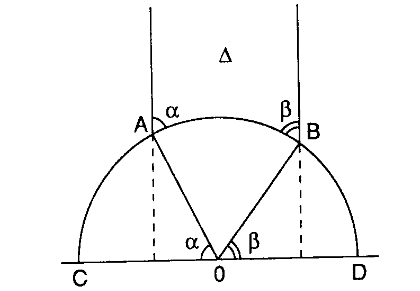
\includegraphics[scale=0.5]{figures/gauss-bonnet.png}
  \caption{Case 1.}
\end{figure}
The area of this triangle can be calculated
\begin{align*}
  \mu(\Delta) &= \int_{\Delta} \f{\dd x \dd y}{y^2}\\
       &= \int^b_a \dd x \int_{\sqrt{1-x^2}}^\infty \f{\dd y}{y^2}\\
       &= \int^b_a \f{\dd x}{\sqrt{1-x^2}}\\
       &= \int_{\pi-\a}^\b \f{-\sin\theta \dd \theta}{\sin\theta}\\
       &= \pi - \a - \b.\\
\end{align*}
\textit{Case 2.} Suppose that none of the vertices are on $\R\cup \{\infty\}$. There exists a transforamtion such that no two vertices lies on a vertical geodesic. Extend the side $AB$, of the triangle $ABC$, to a point $D\in \R$. Let $\Delta_1 = ACD$ and $\Delta_2 = CBD$. Then
\begin{align*}
  \mu(\Delta) = \mu(\Delta_1) - \mu(\Delta_2) = \pi - \a - (\g+\theta) - \pi + \theta + (\pi - \b) = \pi - \a - \b - \g
\end{align*}
\begin{figure}[h]
  \centering
  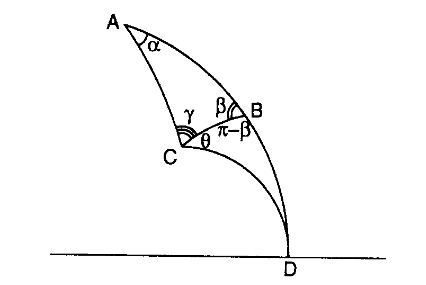
\includegraphics[scale=0.5]{figures/gauss-bonnet-2.png}
  \caption{Case 2.}
\end{figure}
This proves the theorem.
\end{proof}
\begin{corollary}
  The area of an $n-$gon with angles $\a_1\cdots, \a_n$ is $(n-2)\pi - \a_1 - \cdots - \a_n$.
\end{corollary}
\begin{proof}
  This follows from induction. It is true for a trianlge. Suppose it is true for an $n-1$-gon. An $n-$gon can be divided into a triangle and an $n-1$-gon by drawing an appropriate geodesic curve. Adding the areas of the two we get the result.    
\end{proof}
\begin{theorem}[Brouwer's Fixed Point Theorem]
  Let $f: \mathbb{D} \to \mathbb{D}$ be a continous bijection on the disk. There are is atleast one fixed point.
\end{theorem}
\begin{proof}[Amazing proof using Functors]
  Suppose $f$ fixes no point. Define the function $r: \mathbb{D} \to S^1$ in the following way: draw extend the line from $f(x)$ to $x$ to the boundary of $ \mathbb{D}$ where it intersects with the circle at $r(x)$. Note that $r$ fixes each point on $S^1$. We have the short exact sequence
  \[
    \begin{tikzcd}
      0 \arrow[r] & S^1 \arrow[r, "i"]  & \mathbb{D} \arrow[r, "r"]  & S^1 \arrow[r] & 0
    \end{tikzcd}
  \]
  Since there is a functor $ \pi_1: \text{Top}_* \to \text{Grp}$ which maps a based topological space $(X,x_0)$ to it's fundametal group at $x_0$. Applying this functor to the above exact sequence at any point, gives the short exact sequence
  \[
    \begin{tikzcd}
      0 \arrow[r] & \pi_1(S^1) \arrow[r, "\pi_1(i)"]  & \pi_1(\mathbb{D}) \arrow[r, "\pi_1(r)"]  & \pi_1(S^1) \arrow[r] & 0
    \end{tikzcd}
  \]
  Since $\pi_1(S^1) = \Z$ and $\pi_1( \mathbb{D}) = 0$ we get that $\text{id}_{S^1} = \pi_1(r\circ i) = \pi_1(r)\circ\pi_1(i) = 0$, a contradiction. 
\end{proof}
Brouwer's theorem tells us that isometries of $\H$ must fix atleast one point, since $\H$ is isometric to the disk. The following is a classification of
\begin{theorem}
  Let $T$ be an orientation preserving isometry of $\H$. Then one of the following happens:
  \begin{enumerate}
    \item $T$ fixes only one point in $\H$.
    \item $T$ fixes only one point on the boundary of $\H$.
    \item $T$ fixes two points on the boundary of $\H$.
  \end{enumerate}
\end{theorem}
\begin{proof}
  Since $T\in PSL_2(\R)$, $z$ is a fixed point if
  \begin{align*}
    z = \f{az+b}{cz+d} \implies cz^2 + (d-a)z - b = 0
  \end{align*}
  Thus
  \begin{align*}
    z = \f{(a-d) \pm \sqrt{(a+d)^2 -4}}{2c}
  \end{align*}
  Thus case $1$ corresponds to $a+d<2$, $2$ corresponds to $a+d = 2$, and $3$ corresponds to $a+d>2$. 
\end{proof}

\section{Hyperbolic Structures on Surfaces}
For the sake of consistency with the texts, I use the Poincare model of hyperbolic plane here.
\begin{definition}
  Let $X$ be a surface. A hyperbolic structure on $X$ is an atlas of charts such that each chart $\p:U\to \p(U)\subset \H$ is a homeomorphism (equivalently this can be defined to all of $\H$) and the transition maps in the atlas are restrictions of orientation preserving isometries of $\H$.
\end{definition}

Let $p\in X$ and $(U,\p)$ be a chart around $p$. We can define an inner product on $T_p X$ as
\begin{align*}
  \langle u,v \rangle_{T_pX} = \langle \p_* u, \p_* v \rangle  
\end{align*}
This is well defined since if $(V,\psi)$ is another chart containing $p$ then
\begin{align*}
  \langle \psi_* u, \psi_* v \rangle = \langle \psi_*\circ \p_*^{-1}\circ \p_* u, \psi_*\circ\p_*\circ \p_* v \rangle = \langle \p_* u, \p_* v \rangle.
\end{align*}
Since $\langle \cdot, \cdot \rangle_{T_pX}$ is a smooth bilinear map it serves as a Riemann metric on $X$. From here on I drop the subscript $T_pX$ on the metric. The norm induced by the metric will just be written $\|\cdot\|$. From here on we can think of Hyperbolic surface to be a topological surface with a hyperbolic Atlas and a Riemannian metric which is isometric to the hyperbolic metric locally. The metric induces a distance on $X$ which is given by the infimum of the length of the curves.
\begin{proposition}
  Let $\g:[0,1] \to U\subset X$ be a curve in $X$ between $x_0$ and $x_1$. If $\gamma$ is a geodesic then there exist charts $(U_\a,\p_\a)$ such that they cover $\g$ and $\p_\a\circ \g\big|_{U_\a}$ is a segment of a geodesic in $\H$. 
\end{proposition}
\begin{proof}
  Suppose that $\g$ is a geodesic. Let $x$ be a point on $\g$. There exists a neighborhood $U$ of this point which is isometric to $\H$ by the $\p$. Let $\sigma$ be some curve between the end-points of the curve $\p\circ \g$ (which always exist since $\H$ is complete). Then,
  \begin{align*}
    L(\sigma) = L(\p^{-1}\circ \sigma) \geq L(\g) = L(\p\circ\g)
  \end{align*}
  since $\g$ is a geodesic. Thus it follows that $\p\circ \g$ is a geodesic.
\end{proof}

\begin{theorem}[Half of Hopf-Rinow theorem]
  In a complete hyperbolic surface, all geodesics can be extended indefnitely.
\end{theorem}
\begin{proof}
  Suppose that $\g: (-\epsilon, \epsilon)\to X$ is a bounded geodesic in $X$. Then consider a sequence of points $\g(t_n)$ where $t_n \to \e$. Since $X$ is complete the Cauchy sequence $\g(t_n)$ converges to a unique point, say $x_1$. Let $U,\p$ be some chart centered around $x_1$. The image $\p\circ \g$ is a geodesic by previous proposition. Extend this in $\H$ indefnitely. Then the pull back of this extension extends $\g$ at $x_1$ till a new end point $x_2$. Repeating this process one can indefnitely extend $\g$.
\end{proof}
\begin{theorem}
  Any complete, connected, simply-connected hyperbolic surface is isometric to $\H$.
\end{theorem}
\begin{proof}
  Suppose $X$ is a space with the mentioned properties. Consider the maps $E:\H\to X,D:X\to \H$ defined as follows:
  \begin{itemize}
    \item \textit{The exponential.} Choose a point $a\in X$ and a chart $(U, \p)$ such that $\p(a) = 0$. For $x\in \H$ let $\g$ be the geodesic between $0$ and $x$ and then extend the geodesic $\p^{-1}(\g)$. Define $E(x)$ as the point on the extended geodesic such that $\text{dist}(a,E(x)) = \rho(0,x)$.
    \item \textit{The developing.} Fix a point $a\in X$ and a chart $(U,\p)$ around it. There exists a map $D:X\to \H$ such that $D$ is a local isometry and $D\big|_U = \p$. This claim is proven below:
      \begin{proof}[proof of existence of $D$]
        Choose a path $\g$ between points $a,b\in X$. The path can be cover by finitely many convex coordinate charts (due to compactness), say $(U_i,\p_i)$ with $(U_0, \p_0) = (U,\p)$. Refine the covering such that it is minimal (so that $U_i$ only intersects with $U_{i\pm 1}$ and no $U_i$ is contained in $U_j$). Choose points $x_0=a,\cdots,x_i,\cdots,x_n=b$ on $\g$ such that $[x_i,x_{i+1}]\subset U_i$. If the maps $\p_i$ and $\p_{i+1}$ do not agree on $U_i\cap U_{i+1}$, which contains $x_{i+1}$,then there exists an isometry $g$ (unique extension of $\p_{i+1}\circ\p_{i}^{-1}$) such that $g\circ\p_i = \p_{i+1}$ on their intersection. Thus without loss of generality we can assume that all the charts agree on the intersection (by replacing $\p_{i+1}$ with $g\circ \p_1$). Now define $D(b) = \p_n(b)$.\\

        \textit{(Well defined-ness).} Clearly $D$ is not dependent on the choice $x_i$. Now suppose $(U'_i,\p'_i)_{i=0}^m$ is a different set of charts which minimally cover $\g$ with $U_0,\p_0 = U,\p$ and such that the coordinate charts agree on the intersection. We show by induction that whenever $U_i\cap U'_j\neq \emptyset$ then $\p'_j = \p_i$ in the intersection. By construction $U_0 = U_0'$ and $\p'_0 = \p_0$. Since $U'_0\cap U_1 = U_0\cap U_1$ it follows that in this intersection $\p'_0 = \p_0 = \p_1$. This is the base case of the induction. Suppose now that for all $s<j$  if $U'_s\cap U_i \neq \es$ then $\p'_s = \p_i$ in the intersection for all $i$. Consider $U'_j$ and suppose that it intersects with some $U_i$. There are two cases:
        \begin{enumerate}
          \item $U'_{j-1}\cap U_i\neq \es$. In this case consider the intersection $U_i\cap U'_j\cap U'_{j-1}$. In this region $\p'_j= \p'_{j-1} = \p_i$. Restricted to $\p'_j (U_i \cap U'_j)$ the map $g = \p_i\circ (\p'_j)^{-1}$ is in $PSL_2(\R)$. Since on $\p'_j (U_i \cap U'_j \cap U_i)$ the map $g$ is identity it follows that $g$ is identity everywhere in $\p'_j(U_i\cap U'_j)$ (since Mobius maps are fixed by $3$ points). 
          \item $U'_{j-1}\cap U_i = \es$. Then $U'_{j-1}$ intersects $U_{i-1}$ (by construction). In the region $U_{i-1} \cap U_j\cap U_{j-1}$ we have $\p'_j = \p'_{j-1} = \p_{i-1}$ and thus $\p'\circ \p^{-1}_{i-1}$ is identity on infinitely many points. Thus they are the same on $U'_j\cap U_{i-1}$. In the region $U'_j\cap U_i \cap U_{i-1}$ we have $\p'_j = \p_{i-1} = \p_i$. Using the same argument as before we have that $\p_i = \p'_j$ everywhere on $U_i \cap U'_j$.
        \end{enumerate}
        Hence the induction step is complete. Since $b\in U'_m\cap U_n$ it follows that $\p'_m(b) = \p_n(b)$. Hence $D$ is not dependent on the covering of $\g$. Now we need to show that $D$ does not depend on $\g$. If $\g'$ is some other curve. Since $X$ is simply connected it follows that there is a Homotopy $H$ between $\g$ and $\g'$. Using continuity of $H$ there exists an $\e$ so that the curves $H(s,t)$ and $H(s,t+\e)$ can be covered by the same charts. Hence $\p_n(b)$ is the same for both. Thus it follows that $D$ is well defined.
      \end{proof}
  \end{itemize}
  Now that we have these two functions, note that $D\circ E = 1_{\H}$: let $x\in \H$ then $E(x)$ lies on a geodesic $\g$ from $a$ to $E(x)$ such that $\p\circ \g$ is part of the geodesic connecting $0$ and $x$. Let $U_i$ be any minial cover of the geodesic from $a$ to $E(x)$. Then $\p_n(E(x))$ lies on the extension of the geodesic $\p\circ\g$ and $\rho(0,D(E(x))) = \rho(0,x)$ since $D$ and $E$ are local isometries, but there is only one such point on the geodesic: $x$. Hence $D\circ E(x) = x$.\\

  Note that on the image of $E$ in $X$ the map $E\circ D$ is identity. $E(\H)$ is closed and open (since $E$ is local injection it follows by Invariance of domain theorem). Since $X$ is connected the only non-trivial clopen subset is $X$ itself. Thus $E(\H) = X$. Hence $E\circ D = 1_X$.
\end{proof}

As a consequence of the above theorem it follows that the universal cover of any hyperbolic surface $X$ is isometric to $\H$.


% ------------------------------------------------------------------------------
% Reference and Cited Works
% ------------------------------------------------------------------------------
\nocite{*}
\bibliographystyle{IEEEtran}
\bibliography{References.bib}

% ------------------------------------------------------------------------------

\end{document}
